\documentclass[tikz,border=10pt]{standalone}
\begin{document}
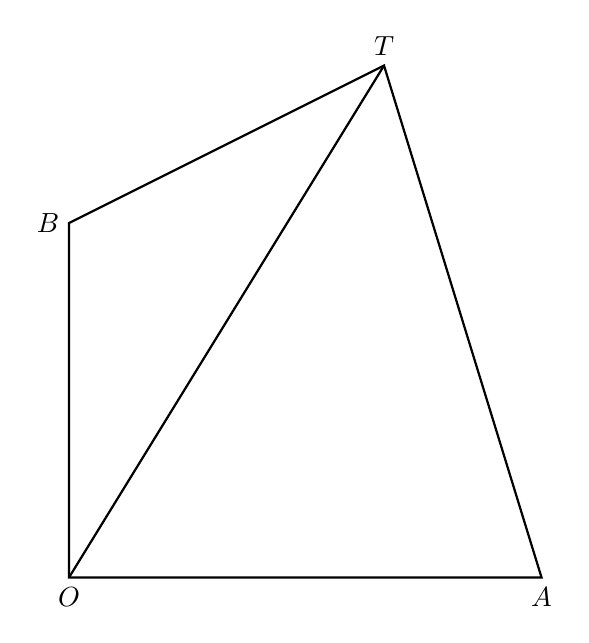
\begin{tikzpicture}
\coordinate (O) at (0,0);
\coordinate (A) at (6,0);
\coordinate (B) at (0,4.5);
\coordinate (T) at (4,6.5);

\draw[thick] (O) -- (A) -- (T) -- (B) -- cycle;
\draw[thick] (O) -- (T);

\node[below] at (O) {$O$};
\node[below] at (A) {$A$};
\node[left] at (B) {$B$};
\node[above] at (T) {$T$};
\end{tikzpicture}
\end{document}
